\documentclass{article}

\usepackage{tikz}
\usepackage{struggle}

\newcommand{\sqrtthree}{(sqrt(3.0))}
\newcommand{\testnode}{(6, 5.454323)}

\begin{document}

\sqrtthree

before

\begin{struggleboard}
  \piece{a1}{red};
  \piece{b1}{blue};
  \arrow{a1}{c1};
\end{struggleboard}
\begin{struggleboard}
\end{struggleboard}

after


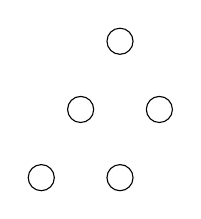
\begin{tikzpicture}
  \tikzstyle{every node}=[draw,circle,minimum size=1pt]
  \node (a1) at (0, 5.196152) {};
  \node (b1) at (-1/2, 4.330127) {};
  \node (b2) at (1/2, 4.330127) {};
  \node (c1) at (-1, 3.4641016) {};
  \node (c2) at (0, 3.4641016) {};
\end{tikzpicture}
hi
\begin{tikzpicture}
  \tikzstyle{every node}=[draw,circle,fill=gray,minimum size=1pt];
  \node (a) at (0, 0) {};
  \node (b) at (1/2, 1.113) {};
  \draw (4, 4.44) circle [radius=1];
  \draw \testnode circle [radius=1];
\end{tikzpicture}

\end{document}